\section*{\textbf{3 - Linear structure growth} \hrule} 



\subsection*{\textbf{Question 3}}
\begin{quote}

\textbf{Problem}
\begin{quote} Solve the ODE of equation \ref{eq:ode}  for the 3 given initial conditions in an matter-dominated Einstein\- de Sitter Universe. Use an appropriate numerical method. Compare the results with the analytical solution of the ODE. Plot the solution for $t = 1$ until $t = 1000$ yr, use a log\- log plot. 
\begin{equation}
\frac{d^2 D}{dt^2} + 2 \frac{\dot{a}}{a} \frac{dD}{dt} = \frac{3}{2} \omega_0 H_0^2\frac{1}{a^3}D
\label{eq:ode}
\end{equation}

\textbf{Initial conditions:}
\begin{equation*}
\text{(1)  } D(1) = 3, D'(1) = 2 \hspace*{1cm} \text{(2)  } D(1) = 10, D'(1) = - 10 \hspace*{1cm} \text{(3) } D(1) = 5, D'(1) = 0
\end{equation*}

\end{quote}

\textbf{Solution} 
\begin{quote}
The solution of this problem consist of three parts. One, a rewritten version of equation \ref{eq:ode} with the scale factor plugged in. Two, a (brief) explanation on how this rewritten version is used numerically. Three, a derivation of the analytical solution.
\\

\textbf{(1) Rewriting the ODE.}
\begin{quote}

The numerical and analytical solution both require a version of equation \ref{eq:ode} with the scale factor plugged in. For an Einstein-de Sitter Universe the scale factor and its derivative are given by, 
\begin{equation}
a(t) = \left(\frac{3}{2} H_0 t \right)^{2/3} \hspace*{1cm} \text{and} \hspace*{1cm} \dot{a}(t) = H_0 \left(\frac{3}{2} H_0 t \right)^{-1/3}
\end{equation}

Plugin this in by equation \ref{eq:ode} and using that $\Omega_0 = 1$  yields the rewritten version of equation \ref{eq:ode},
\begin{align}
\frac{d^2D}{dt^2} + \frac{H_0 \left(\frac{3}{2} H_0 t \right)^{-1/3}}{\left(\frac{3}{2} H_0 t \right)^{2/3}} \frac{dD}{dt} - \frac{3}{2} \Omega_0 \frac{H_0^2}{\left(\frac{3}{2} H_0 t \right)^{2/3}}D &= 0 \\
\frac{d^2D}{dt^2} + \frac{4}{3t} \frac{dD}{dt} - \frac{2}{3t^2}D &= 0
\label{eq:ode2}
\end{align}
\end{quote}

\textbf{(2) Numerical solution}
\begin{quote}
The numerical solution is obtained by first writing equation \ref{eq:ode2} as a system of first order ODE's and then by applying the Dormand\- Prince version of the Runde kutta method to solve it. The second order ODE  can be written as a system of first order ODE's by substituting $dD/dt = u$. The system then becomes,

\begin{equation}
\large
\begin{cases} 
\frac{dD}{dt} &= u \\ 
\frac{d^2D}{d^2} &= - \frac{4}{3t}u + \frac{2}{3t^2}D 
\end{cases}
\end{equation}

The above system is as mentioned before solved with the Dormand\- Prince version of the Runde kutta method. The algorithm uses an adaptive step size that is initial set to $t_{step} = 0.01$ year for all cases. The obtained results c an be found on page .....
\end{quote}

\textbf{(3) Analytical solution}
\begin{quote}
The analytical solution that is required for the plots can be found by solving equation \ref{eq:ode2}. The equation is solved by finding two particular solutions. These can be found by finding the values of lambda for which the the ansatz $D(t) = t^{\lambda}$ holds. Plugin in the ansatz yields,

\begin{equation}
\lambda \left(\lambda -1 \right) t^{\lambda - 2} + \frac{4}{3t} \lambda t^{\lambda -1} - \frac{2}{3t^2}t^{\lambda} = 0
\end{equation}

This simplifies to
\begin{align*}
0 & = \lambda \left( \lambda -1 \right) t^{\lambda} + \frac{4}{3} \lambda t^{\lambda} - \frac{2}{3} t^{\lambda}  \\
&= \lambda ( \lambda -1 ) + \frac{4}{3} \lambda - \frac{2}{3}  \\
&= \lambda^2 + \frac{1}{3} \lambda - \frac{2}{3} \\
&= (\lambda + 1) (\lambda - \frac{2}{3} )  \\
\end{align*}

The peculiar solutions of the ODE are thus given by,
\begin{equation}
D(t) = t^{-1} \hspace*{2cm} D(t) = t^{2/3}
\end{equation}

The general solution is the super position of the peculair solutions  and can therefore be written as,
\begin{equation}
D(t) = c_{1} t^{2/3} + c_2 t^{-1}
\end{equation}

The constants for the three initial cases can be found by calculating the derivative of the above equation and plugin in t he initial conditions. This yields for the three cases that, %Calculating the derivative and plugin in the inital conditions for the three cases, yields the values was The constants are dependent on the inital conditions. Plugin in the initial conditons for the three cases and solving the system yields the values,

\begin{equation}
\text{(1) } c_1 = 3, c_2 = 0 \hspace*{1cm} \text{(2) } c_1 =0, c_2 = 10, \hspace*{1cm} \text{(3) } c_1 = 3, c_2 = 2 
\end{equation}

\end{quote}

The code that is used to solve the ODE numerically and generates the plots is split over two files. The first file generates the plots and the second file contains the implementation of the Kunde gutta method. The code and its output can be found below. % can be found below. The code  
\end{quote}

\textbf{Code}

\begin{quote}
The code for generating the three plots.
\centering
\lstinputlisting{./Code/assigment_3.py}
\end{quote}

The code for the Runde kutta method
\centering
\lstinputlisting{./Code/mathlib/ode.py}
\newpage

\textbf{Code - Output plot(s)}
\begin{quote}
\begin{figure}[!ht]
\centering
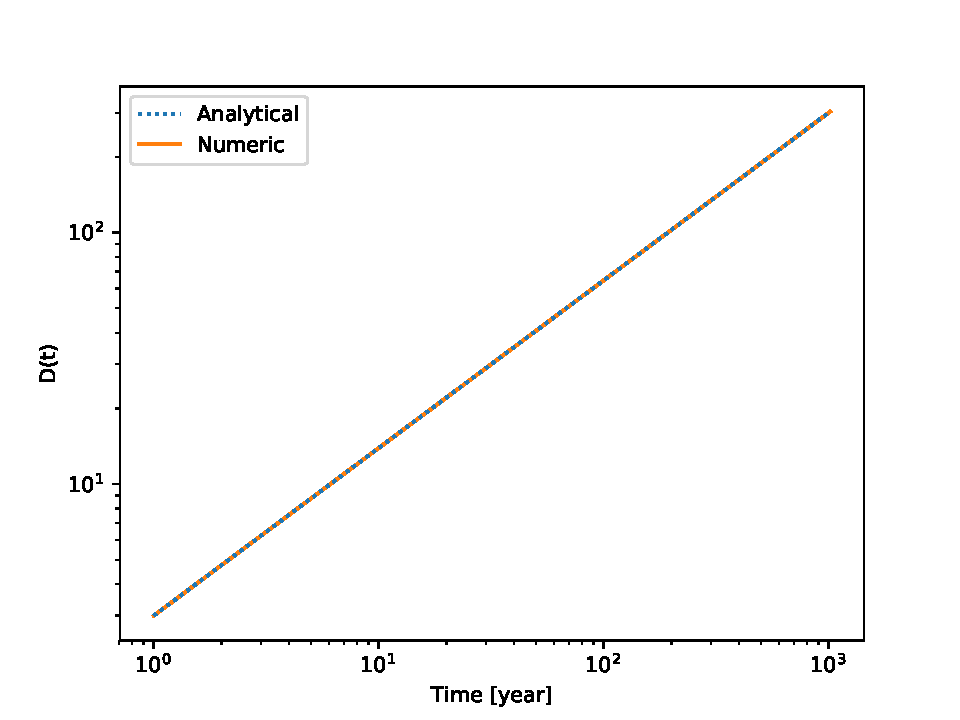
\includegraphics[width=12cm, height=7.5cm]{./Plots/3_ode_0.pdf}
\caption{TODO}
\end{figure}

\begin{figure}[!ht]
\centering
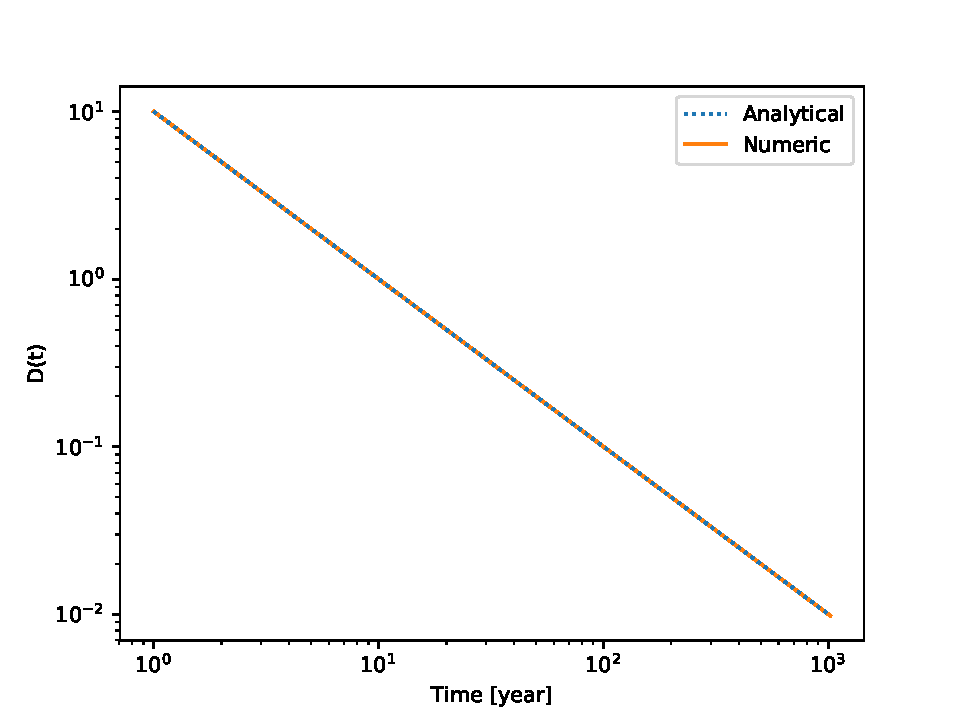
\includegraphics[width=12cm, height=7.5cm]{./Plots/3_ode_1.pdf}
\caption{TODO}
\end{figure}

\begin{figure}[!ht]
\centering
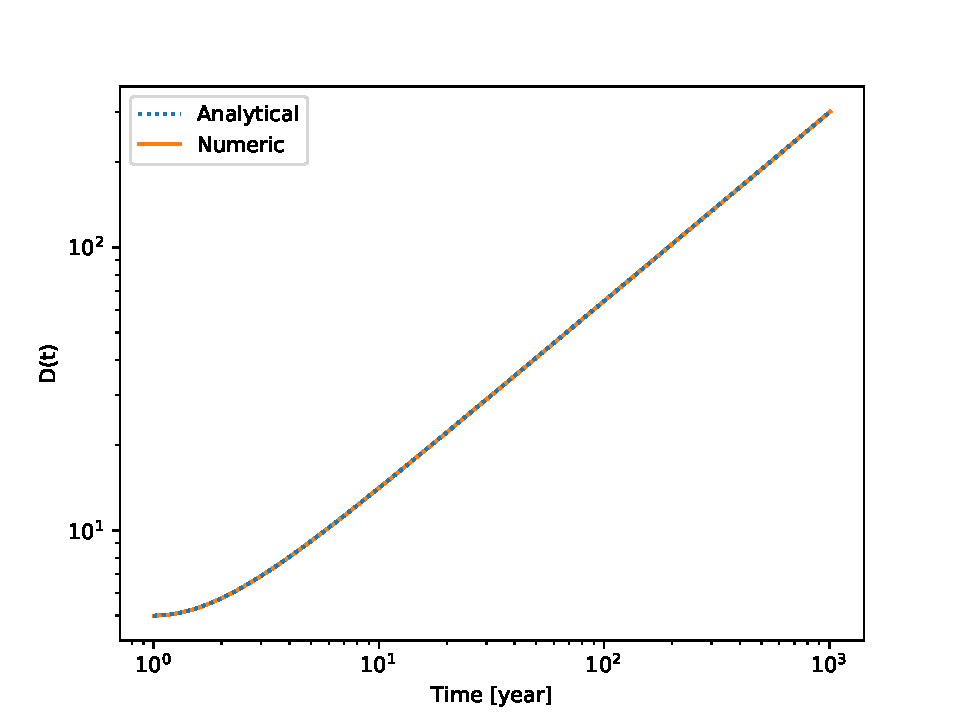
\includegraphics[width=12cm, height=7.5cm]{./Plots/3_ode_2.pdf}
\caption{TODO}
\end{figure}

\end{quote}
\end{quote}






